\section{Statistical analysis}
\label{sec:statistical_analysis}

The statistical analysis of the results proceeds using the frequentist
framework presented in~\Cref{sec:statistical_methods} to search for
non-resonant production of SM \HH and production via scalar resonances
with masses ranging from \SIrange{251}{1600}{\GeV}.

A probabilistic model is constructed targeting the signal hypothesis
to be probed that simultaneously describes the data in bins of the MVA
descriminants in the signal regions and \mll in the \ZHF control
region using the signal and background estimates and their
uncertainties described in earlier sections. The discriminants are
summarised in~\Cref{tab:fitted_variable} for all regions entering the
models for the SM and BSM search.

\begin{table}[htbp]
  \centering
  \begin{tabular}{lccccc}
    \toprule
    & \multicolumn{4}{c}{Discriminant used in channel} \\
    \cline{2-5}
    Search & \hadhad & \lephad SLT & \lephad LTT & \ZHF CR \\
    \midrule
    Non-resonant SM \HH & BDT & NN & NN & \mll \\
    Resonant $X \to \HH$ & PNN (\mX) & PNN (\mX) & PNN (\mX) & \mll \\
    \bottomrule
  \end{tabular}
  \caption{Summary of the types of discriminants used in the binned
    likelihood fits in the three signal regions and the control
    region. The search for resonant production of Higgs boson pairs
    uses the PNN distribution evaluated with a mass parameter equal to
    the resonance mass to be probed.}
  \label{tab:fitted_variable}
\end{table}

The parameters of interest (POI) for the search for non-resonant SM
\HH production are the cross section of the combination of the ggF and
VBF production modes, \xsecggfvbf, and the signal strength
\begin{align*}
  \mu = \frac{\xsecggfvbf}{\xsecggfvbf^{\text{SM}}} \,\text{,}
\end{align*}
which measures the cross section relative to the Standard Model
prediction
of~$\xsecggfvbf^{\text{SM}} = \SI{31.05}{\femto\barn} \text{ (ggF)} +
\SI{1.726}{\femto\barn} \text{
  (VBF)}$~\cite{Grazzini:2018bsd,Dreyer:2018qbw}. In the BSM scenario
of resonant production of Higgs boson pairs via scalar resonances,
only the total cross section of $\sigma(pp \to X \to HH)$ is
considered as the POI. Moreover, the non-resonant production of SM \HH
is not considered as a background in the search for scalar resonances
as there is no experimental evidence for its existence yet.

In the following, the details of the signal and background model are
described in~\Cref{sec:sig_bkg_model}. In~\Cref{sec:results_nonres}
and~\Cref{sec:results_res} the results are presented.
% after performing model parameter estimation using the maximum
% likelihood method and performing likelihood ratio tests to compare
% competing hypothese.

\todo[inline]{Chapter with validation plots before this one?}

\subsection{The signal and background model}%
\label{sec:sig_bkg_model}

The signal and background model describes the expected number of
events in bins .

The sensitivity to a given signal depends due to the use of MVA
discriminants (cf.\ \Cref{tab:fitted_variable})

The use of MVA discriminants in the statistical analysis .

The binning of data in the \ZHF control region is the same in all
cases (cf.\ REFERENCE).


The model described in the following is to be used in a simultaneous
maximum likelihood fit of binned MVA discriminants.

For every signal hypothesis dedicated models are constructed.

The signal considered for non-resonant SM \HH search are ggF+VBF.

\todo[inline]{Simultaneous maximum likelihood fit of binned MVA
  discriminants and control regions to estimate the model parameters.}

The statistical uncertainties on the background prediction using
simulation and control region data are implemented in the likelihood
model according to the simplified Barlow-Beeston method introduced
in~\Cref{sec:barlow_beeston}.

\todo[inline]{Reminder of freely floating backgrounds}
\todo[inline]{Emphasise that there are really many models for each MVA score that is fit.}
\todo[inline]{Models developed in a blind analysis (blind -> high MVA score region blinded)}
\todo[inline]{Maybe say something about blinding?}

\subsubsection{Re-binning algorithm}%
\label{sec:binning_alg}

The signal sensitivity of likelihood-ratio tests using binned MVA
score distributions depends on the choice of binning used for the
discriminant. The purity of signal increases with increasing MVA
score, with most signal (background) being concentrated at the highest
(lowest) scores. For good expected signal sensitivity, the binning has
to be chosen such that regions in MVA score with low
signal-to-background ratio are separated from regions with high
signal-to-background ratio.

In this analysis an iterative re-binning algorithm is used to
determine the binning of MVA discriminants used to construct the
likelihood functions. The aim of the algorithm is to provide large
expected signal sensitivity while ensuring that the background
prediction obeys predefined constraints on the statistical uncertainty
and expected number of events in each bin. The constraints are
intended to stabilise the fits and ensure validity of asymptotic
approximations of the sampling distributions of the test statistics
used in the analysis. The algorithm described in the
following was previously used in Ref.~\cite{HIGG-2016-16-witherratum}
and is continued to be used in the \hadhad channel of this search. A
different algorithm, while conceptually similar, is used in the
\lephad channels and is described in Ref.~\cite{ATLAS-CONF-2021-030}.

The re-binning algorithm is provided with MVA score histograms with
fine, equidistant binning ($N_\text{bins} = 1000$) of the signal and
total background expectation at the nominal values of all nuisance
parameters. It proceeds by iteratively merging bins, starting from the
most-signal like MVA score bins, until the bin fulfills a set of
requirements:
\begin{enumerate}

\item The relative statistical uncertainty of the background
  prediction in the bin must be smaller
  than~\mbox{$\SI{50}{\percent} \times f_\text{s} +
    \SI{1}{\percent}$}, where $f_\text{s}$ is the fraction of signal
  events in the bin relative to the total number of signal events in
  the considered region.  This requirement limits the statistical
  uncertainty of the background estimate in the most signal-like bins
  after re-binning to be in the range of \SIrange{10}{20}{\percent}.

\item The expected number of background events in the bin must be
  larger than 5.

\end{enumerate}
When a bin fulfilling all requirements is found, the process is
repeated starting from the next bin that is not yet merged. The
algorithm terminates with a final bin at low MVA score. If the final
bin does not fulfil the criteria, it is merged with the preceeding
bin.

The size of bins resulting from the re-binning procedure can vary by
multiple orders of magnitude. For better visualisation of the bin
contents, the MVA scores are displayed as equidistant bins.

% The algorithm provides a binning that improves the analysis
% sensitivity while fulfilling criteria on the background model:
% I.e. that it has reasonable statistical precision, and that one
% expects at least 5 events so that asymptotic approximations of the
% test statistics can be used.

% Motivation of terms: 1\% have some bins in background dominated
% region signal fraction weighted 50\% to have relatively fine bins in
% the most signal-like regions


\subsubsection{Merging of physics processes}

The signal and background models are simplified by merging samples
originating from similar underlying physics processes which are
subject to equal treatment in the fit model. In the SM \HH search, the
ggF and VBF samples are merged, defining the total signal contribution
from both production modes. The \Zjets samples are combined into
$Z + (bb,bc,cc)$ and $Z + (bl,cl,ll)$ samples, separately for
$Z \to \tau\tau$ and $Z \to \ell^+\ell^-$, where $\ell = e,
\mu$. Further, contributions from diboson and single top production
(including $tW$) are merged into two separate samples.

The treatment merging for \faketauhadvis backgrounds differs between
the \hadhad and \lephad channels. In the \hadhad channel two separate
samples are used for \tauhadvis background from multi-jet and \ttbar
production. In \lephad channels, all \faketauhadvis contributions are
merged since the estimation method does not distinguish between the
\faketauhadvis source.

The merging of samples should not have a large effect on the
statistical analysis. The only differences arise from symmetrisation,
smoothing, and pruning algorithms (discussed in the following) acting
on merged samples instead of the initial components.


\subsubsection{Symmetrisation of systematic uncertainties}

Uncertainties arising from MC-to-MC comparisons, for example for
alternative generator configurations (e.g.\ variations of the ME or PS
generation), provide only a single systematic variation and thus
cannot be readily incorporated into the likelihood function using a
Gaussian constraint term for the associated uncertainty. These
\emph{one-sided uncertainties} are therefore symmetrised by mirroring
their effect with respect to the nominal prediction. This procedure is
used for all uncertainties resulting from a comparison with a single
alternative prediction.

For some uncertainties the $+1\sigma$ and the $-1\sigma$ variation
changes the prediction in one or multiple bins in the same direction
with respect to the nominal prediction. For such cases, examples being
jet-related uncertainties affecting the four-momenta of reconstructed
jets, the uncertainties are symmetrised by assigning half of the
difference between the up and down variations as a symmetric
uncertainty on the nominal prediction.


\subsubsection{Inter- and extrapolation of systematic uncertainties}

To define a (continuous) likelihood function, the signal and
background predictions have to be parametrised as continuous functions
of the nuisance parameters. Conventionally, uncertainties on the
normalisation or the normalisation and shape of a prediction in a
given analysis region are determined only for two values of the
nuisance parameters correponding to $\pm 1\sigma$ ($\alpha = \pm 1$)
variations in addition to the nominal prediction. The parametrised
predictions needed for the definition of the likelihood function are
obtained using interpolation ($\vert \alpha \vert \leq 1$) and
extrapolation methods ($\vert \alpha \vert > 1$) provided by
\textsc{HistFactory}~\cite{cranmer2012}.

All uncertainties are decomposed into two correlated components
employing different inter- and extrapolation methods. The first
component are uncertainties on the sample normalisations in a given
region which are parametrised using multiplicative normalisation
factors determined from 6th order polynomial interpolation and
exponential extrapolation in $\alpha$. Exponential extrapolation is
used to prevent the normalisation factors from becoming negative. The
second component are shape variations of the discriminant in a given
region that leave the normalisation invariant. The parametrised shape
variations are obtained using 6th order polynomial interpolation and
linear extrapolation. In both cases the resulting functions are
required to be continuous and have continuous first and second
derivatives at the boundaries.


\subsubsection{Smoothing and pruning of systematic uncertainties}

The derivation of shape uncertainties are susceptible to statistical
fluctuations\footnote{This is can also be the case for normalisation
  uncertainties which are not the subject of the smoothing
  algorithm. In this case the user is responsible to ensure that
  normalisation uncertainties are determined with sufficient
  precision.} which can introduce spurious pulls and constraints on
nuisance parameters when performing maximum likelihood fits of the
model. Frequently this is the case when shape uncertainties are
derived from MC-to-MC comparisons or from variations that change the
four-momentum of final state particles. In these cases a smoothing
procedure is applied to the templates describing the uncertainties on
the shape of the discriminant. Shape uncertainties that are based on
the reweighting of the nominal prediction are less sensitive to
statistical fluctuations, unless the weight distribution has high
variance, and thus no smoothing is applied by default. Exceptions are
made in some cases for example for the weight-based FSR uncertainties
for the production of top quarks for which smoothing is applied due to
the large variance of the associated weight distribution.

The smoothing procedure, adopted from Ref.~\cite{HIGG-2013-23}, uses
iterative rebinning of the histogram-based templates describing the
shape uncertainties, merging bins starting with bins that are most
compatible until the statistical uncertainty in all bins is below
\SI{5}{\percent} and the shape template has a monotonic
dependency\todo{Why?} on the (MVA) discriminant. This procedure is
applied, when configured for a given uncertainty, separately for all
analysis regions and samples after merging.

The signal and background model is further simplified by removing
small systematic variations. This pruning procedure is applied
separately for all samples and analysis regions after merging,
symmetrisation, and smoothing. Additionally, uncertainties on the
normalisation and shape are pruned separately. The normalisation
component of an uncertainty for a given sample and analysis category
is removed if both the $+1\sigma$ and $-1\sigma$ variations are within
\SI{0.5}{\percent} with respect to the nominal prediction. The shape
component of an uncertainty is removed if both the $+1\sigma$ and
$-1\sigma$ variations results in changes within \SI{0.5}{\percent} of
the nominal prediction in all bins in the analysis region.


\subsubsection{Nuisance parameter correlation scheme}
\subsubsection{Model validation}





\subsection{Results of the search for non-resonant production of SM $HH$}
\label{sec:results_nonres}


\begin{figure}[htbp]
  \centering

  \begin{subfigure}{0.495\textwidth}
    \centering

    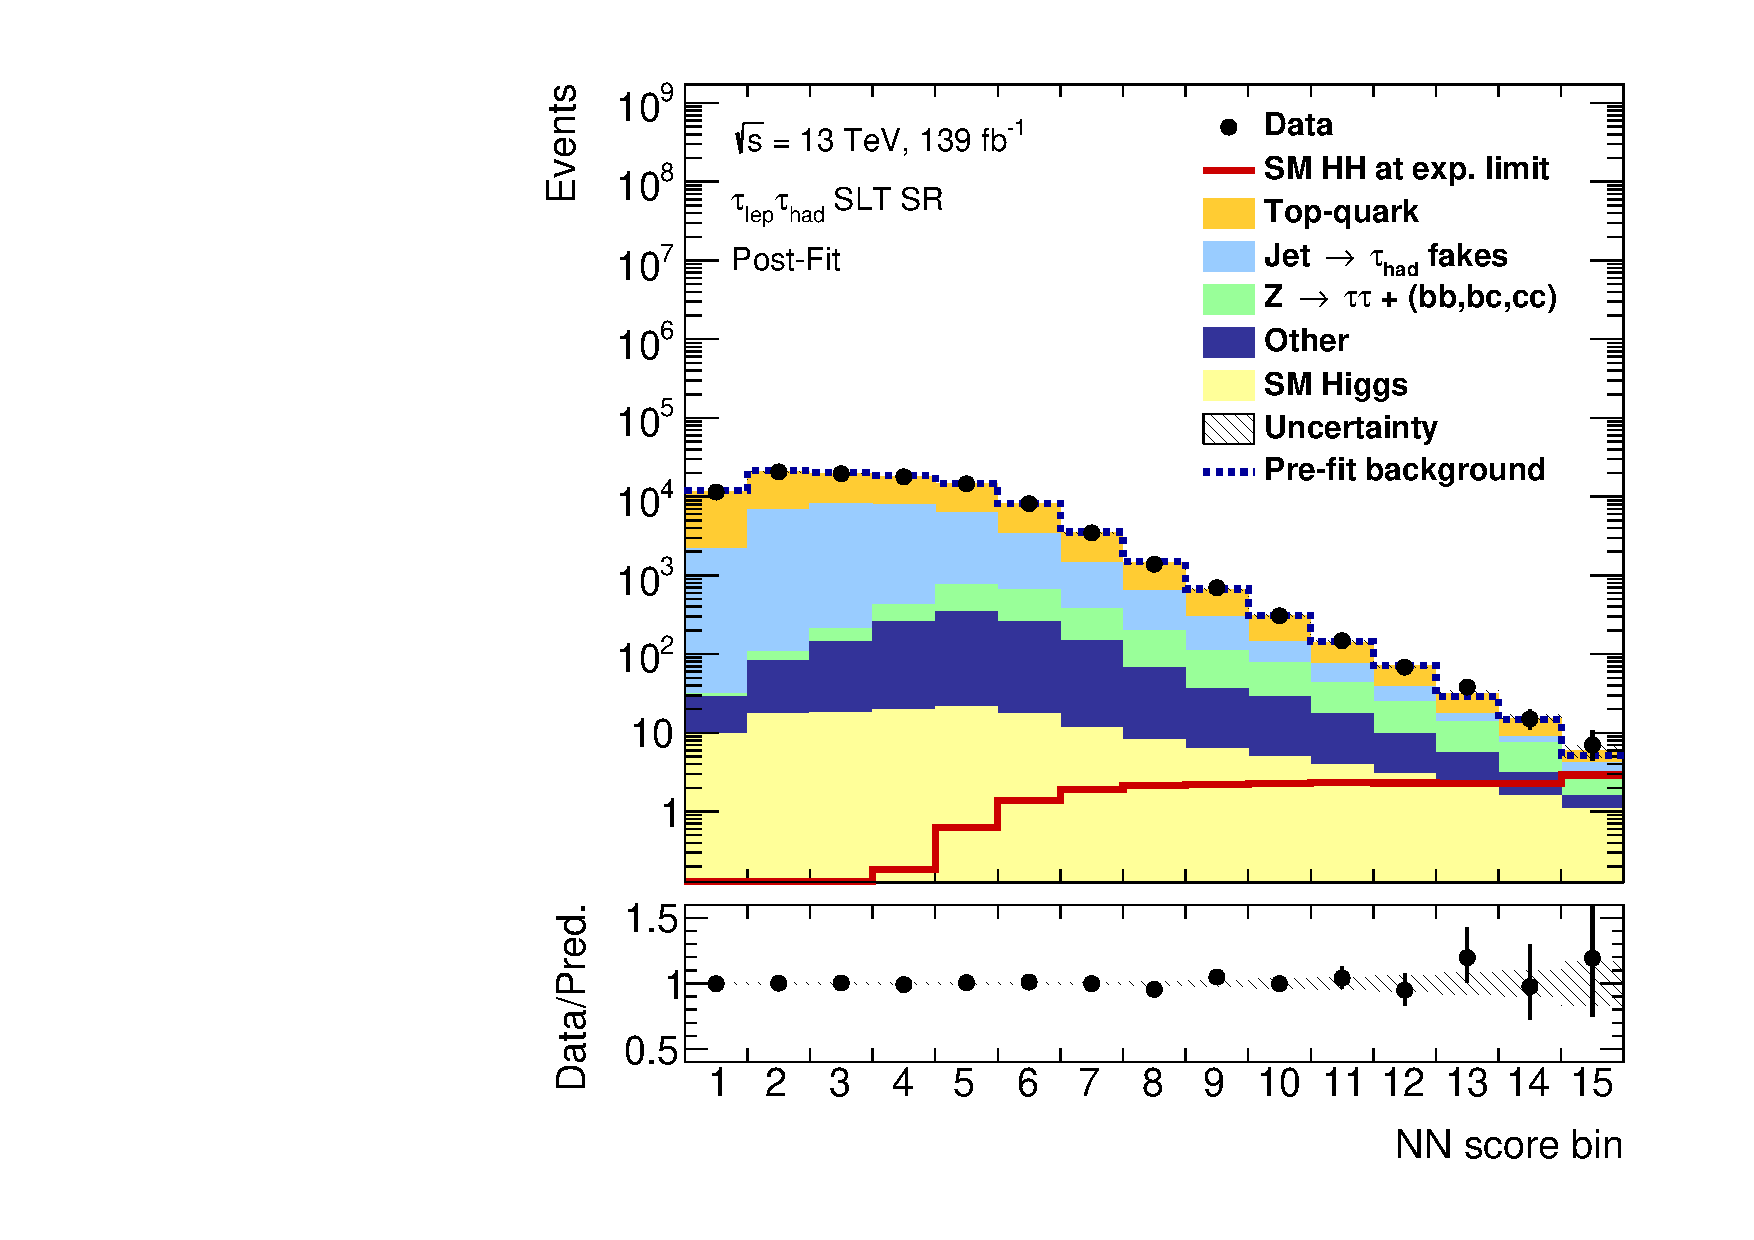
\includegraphics[width=\textwidth]{results_nonres/postfit/Region_BMin0_incJet1_distNN_J2_DSM_T2_SpcTauLH_Y2015_LTT0_L1_GlobalFit_conditionnal_mu0log}

    \subcaption{\lephad SLT channel}
  \end{subfigure}\hfill%
  \begin{subfigure}{0.495\textwidth}
    \centering

    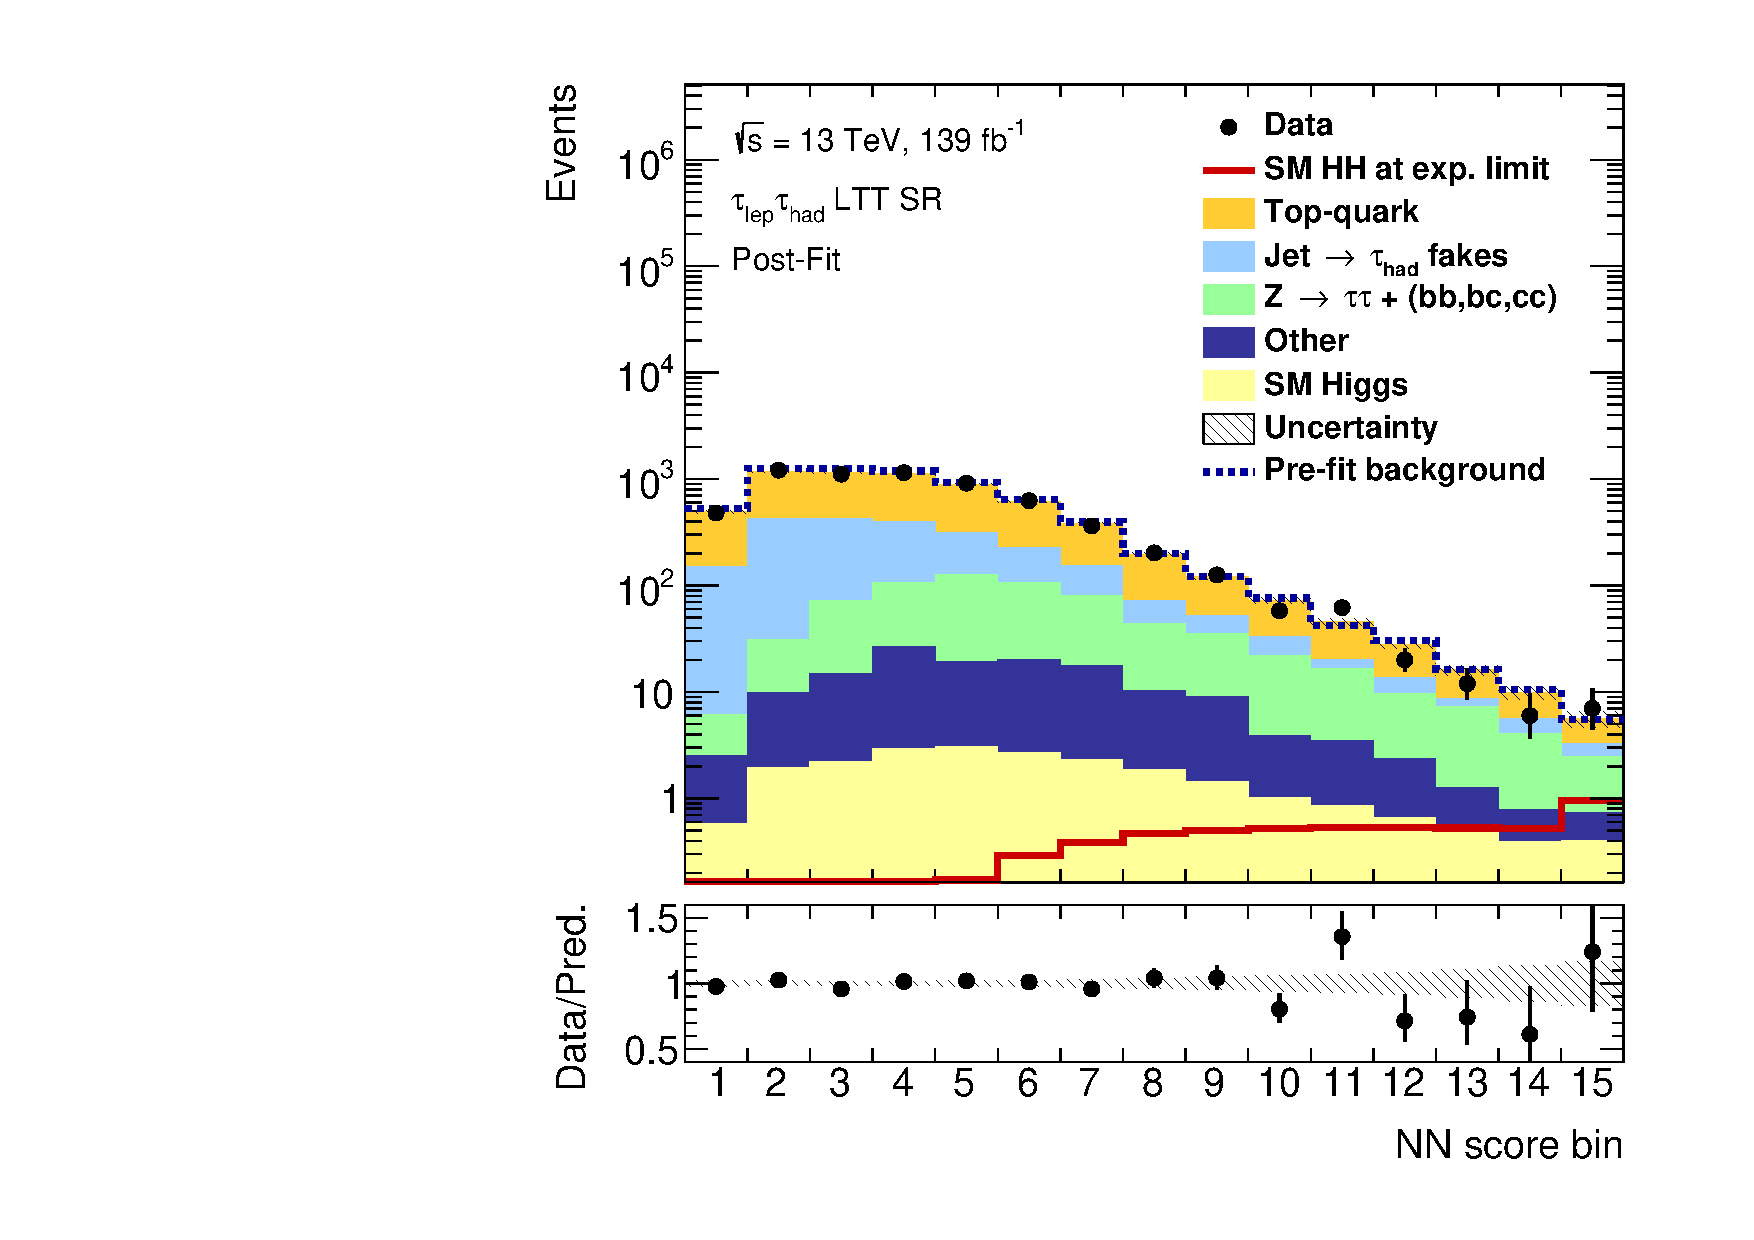
\includegraphics[width=\textwidth]{results_nonres/postfit/Region_BMin0_incJet1_distNN_J2_DSM_T2_SpcTauLH_Y2015_LTT1_L1_GlobalFit_conditionnal_mu0log}

    \subcaption{\lephad LTT channel}
  \end{subfigure}

  \vspace{0.5em}

  \begin{subfigure}{0.495\textwidth}
    \centering

    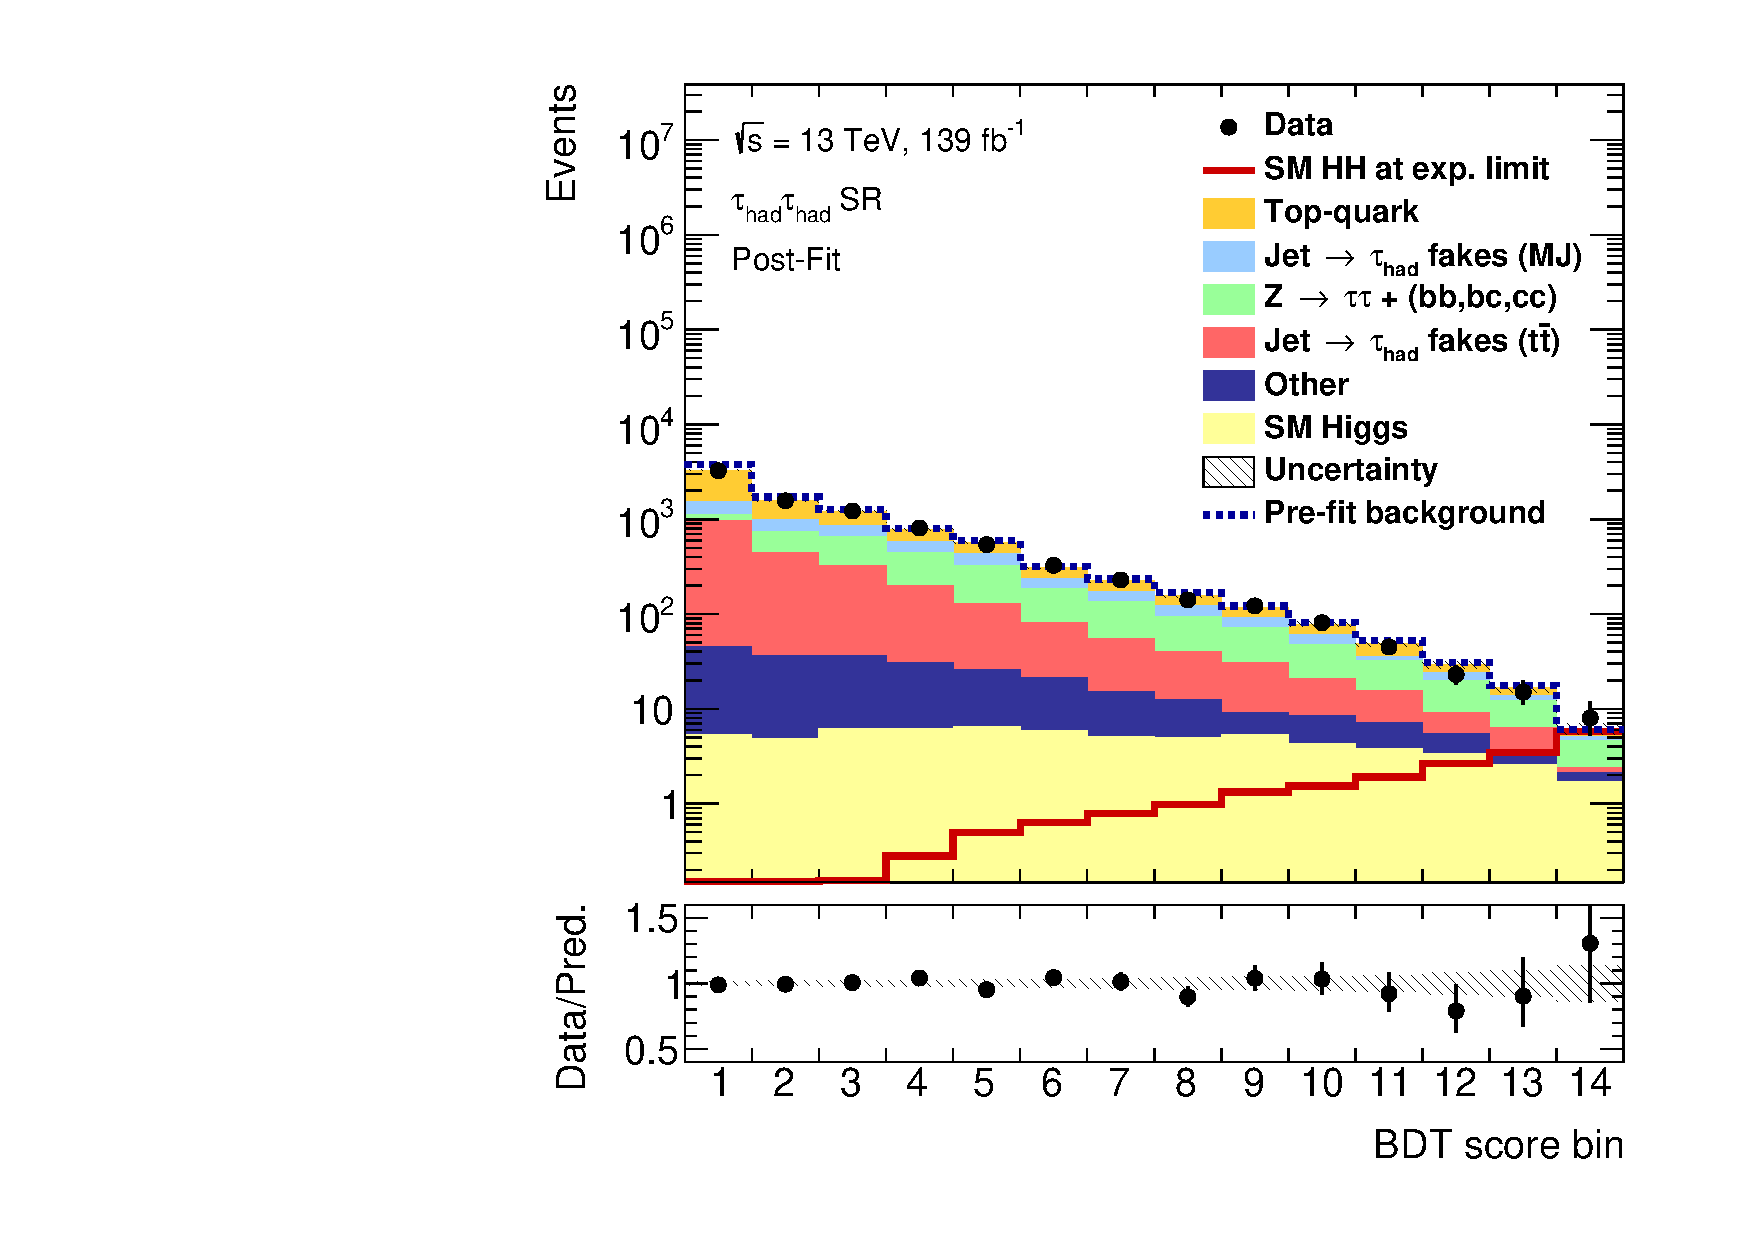
\includegraphics[width=\textwidth]{results_nonres/postfit/Region_BMin0_incJet1_distSMBDT_J2_Y2015_DLLOS_T2_SpcTauHH_L0_GlobalFit_conditionnal_mu0log}

    \subcaption{\hadhad channel}
  \end{subfigure}

  \caption{Distribution of the MVA discriminants used to extract the
    non-resonant SM \HH signal in the \lephad SLT (a), \lephad LTT
    (b), and \hadhad (c) channel after the background-only fit of all
    signal and control regions. The signal overlay is scaled to the
    expected upper limit on the signal strength of $3.9$ from the
    combination of all channels.}
\end{figure}



\begin{figure}[htbp]
  \centering

  \begin{subfigure}{0.46\textwidth}
    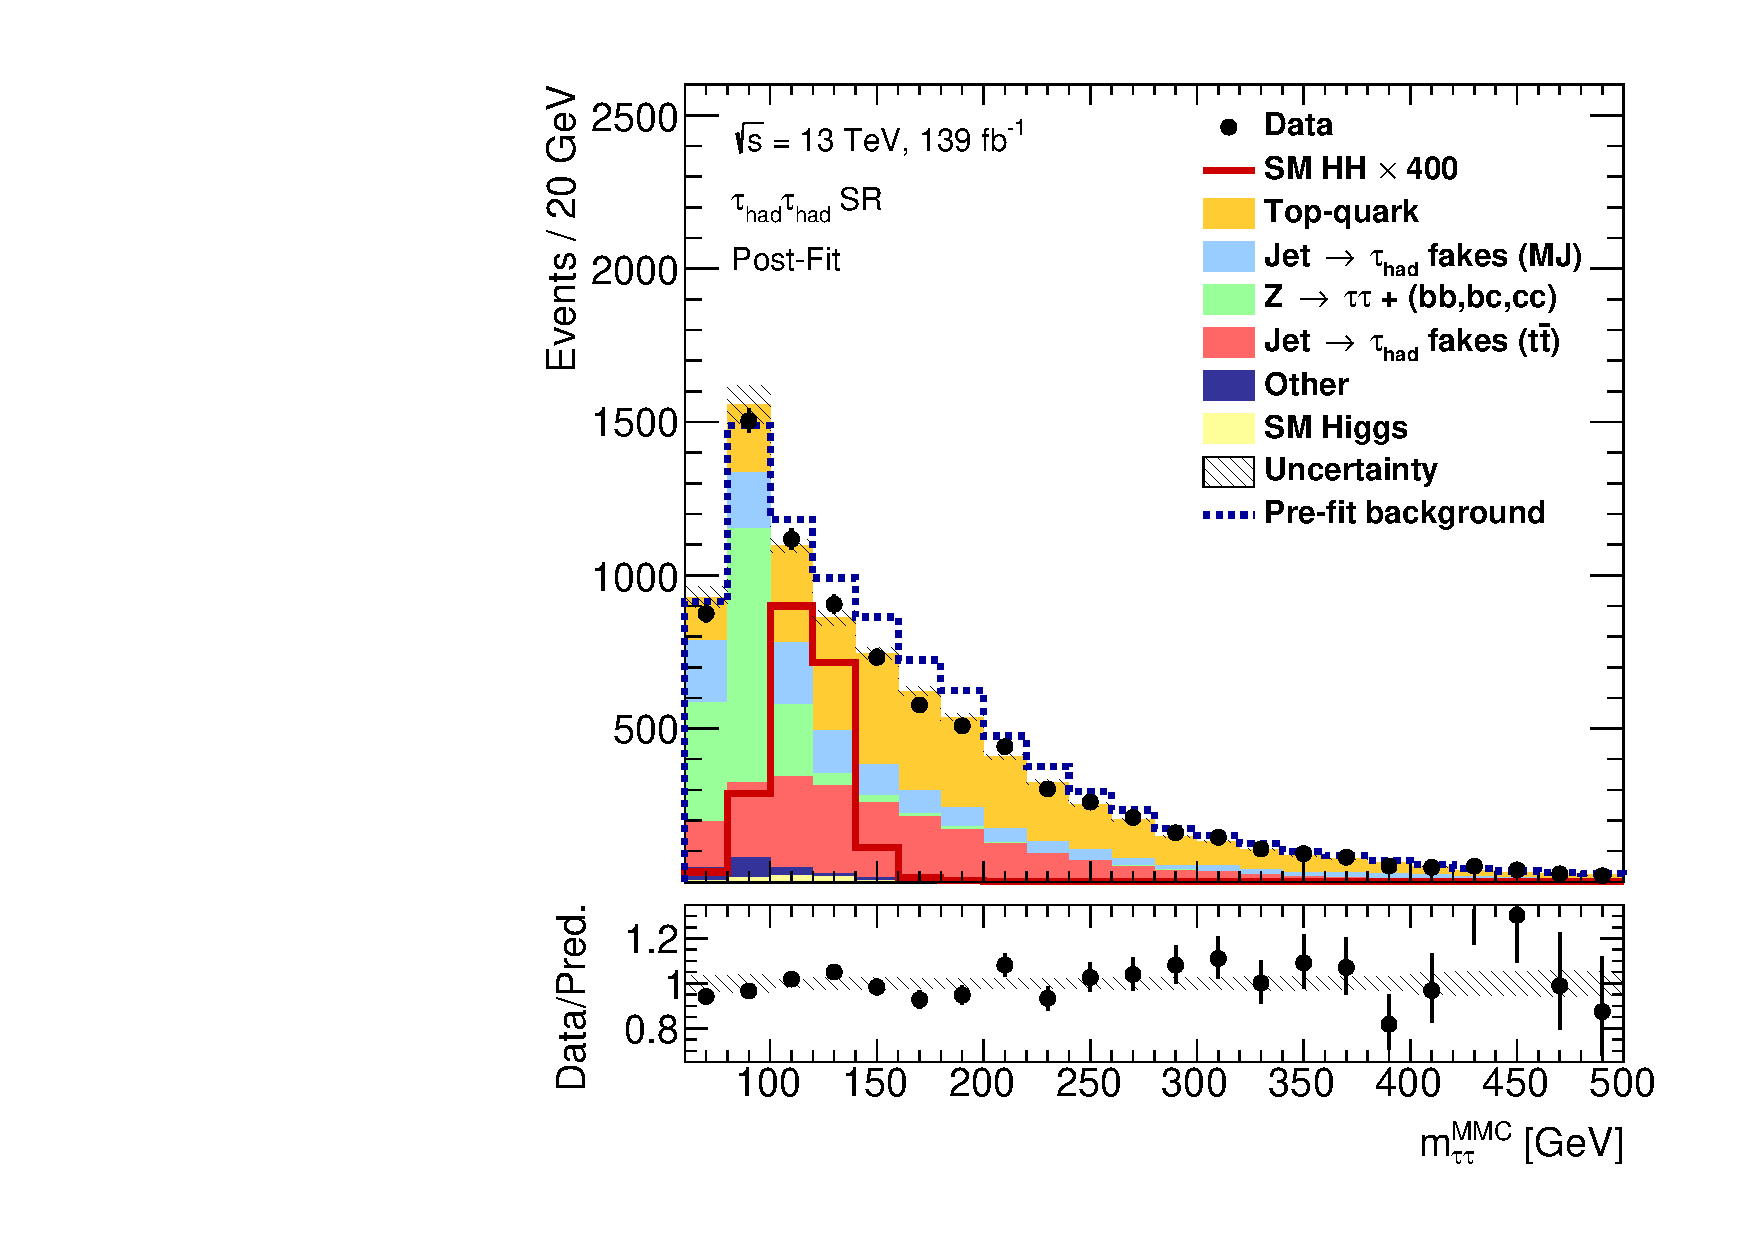
\includegraphics[width=\textwidth]{results_nonres/postfit_mvainputs/Region_BMin0_incJet1_distmMMC_J2_Y2015_DLLOS_T2_SpcTauHH_L0_GlobalFit_conditionnal_mu0}
  \end{subfigure}\hfill%
  \begin{subfigure}{0.46\textwidth}
    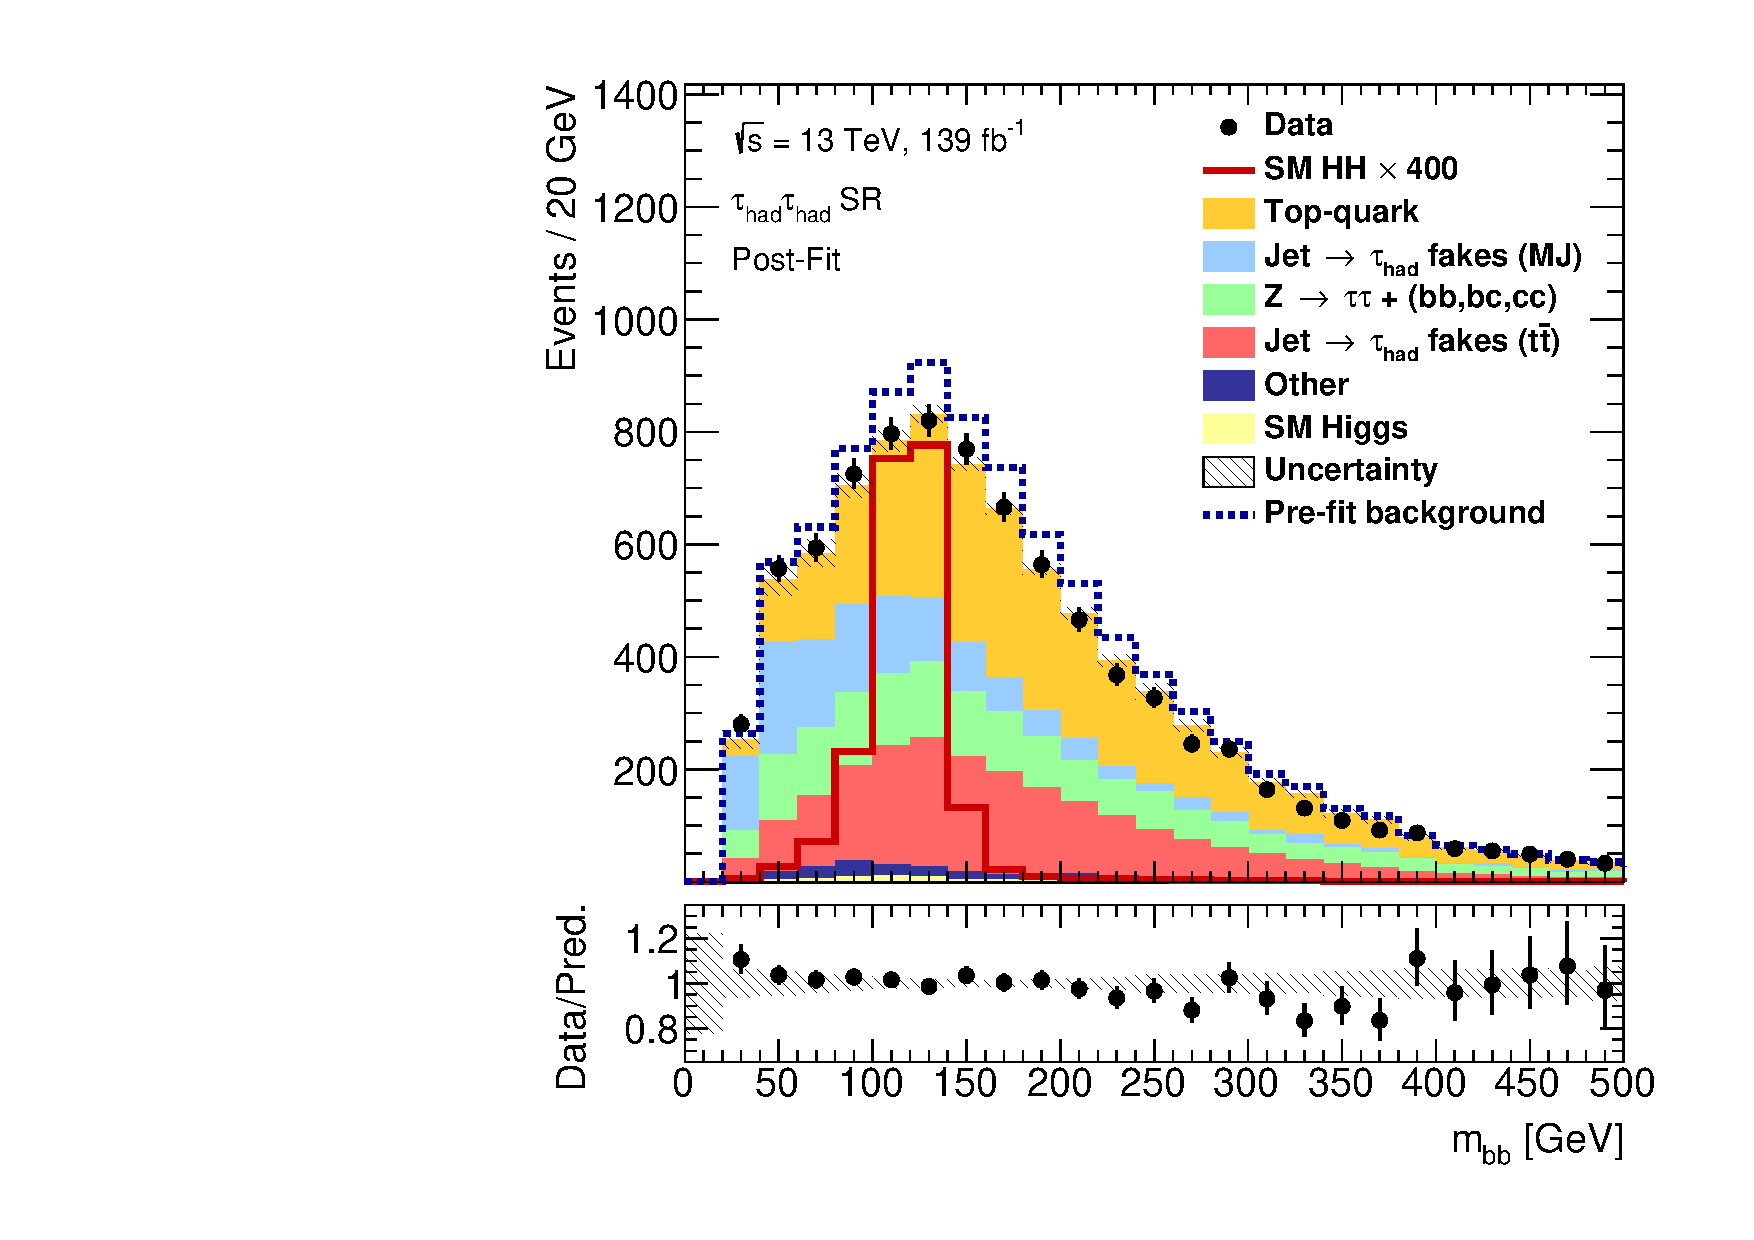
\includegraphics[width=\textwidth]{results_nonres/postfit_mvainputs/Region_BMin0_incJet1_distmBB_J2_Y2015_DLLOS_T2_SpcTauHH_L0_GlobalFit_conditionnal_mu0}
  \end{subfigure}

  \begin{subfigure}{0.46\textwidth}
    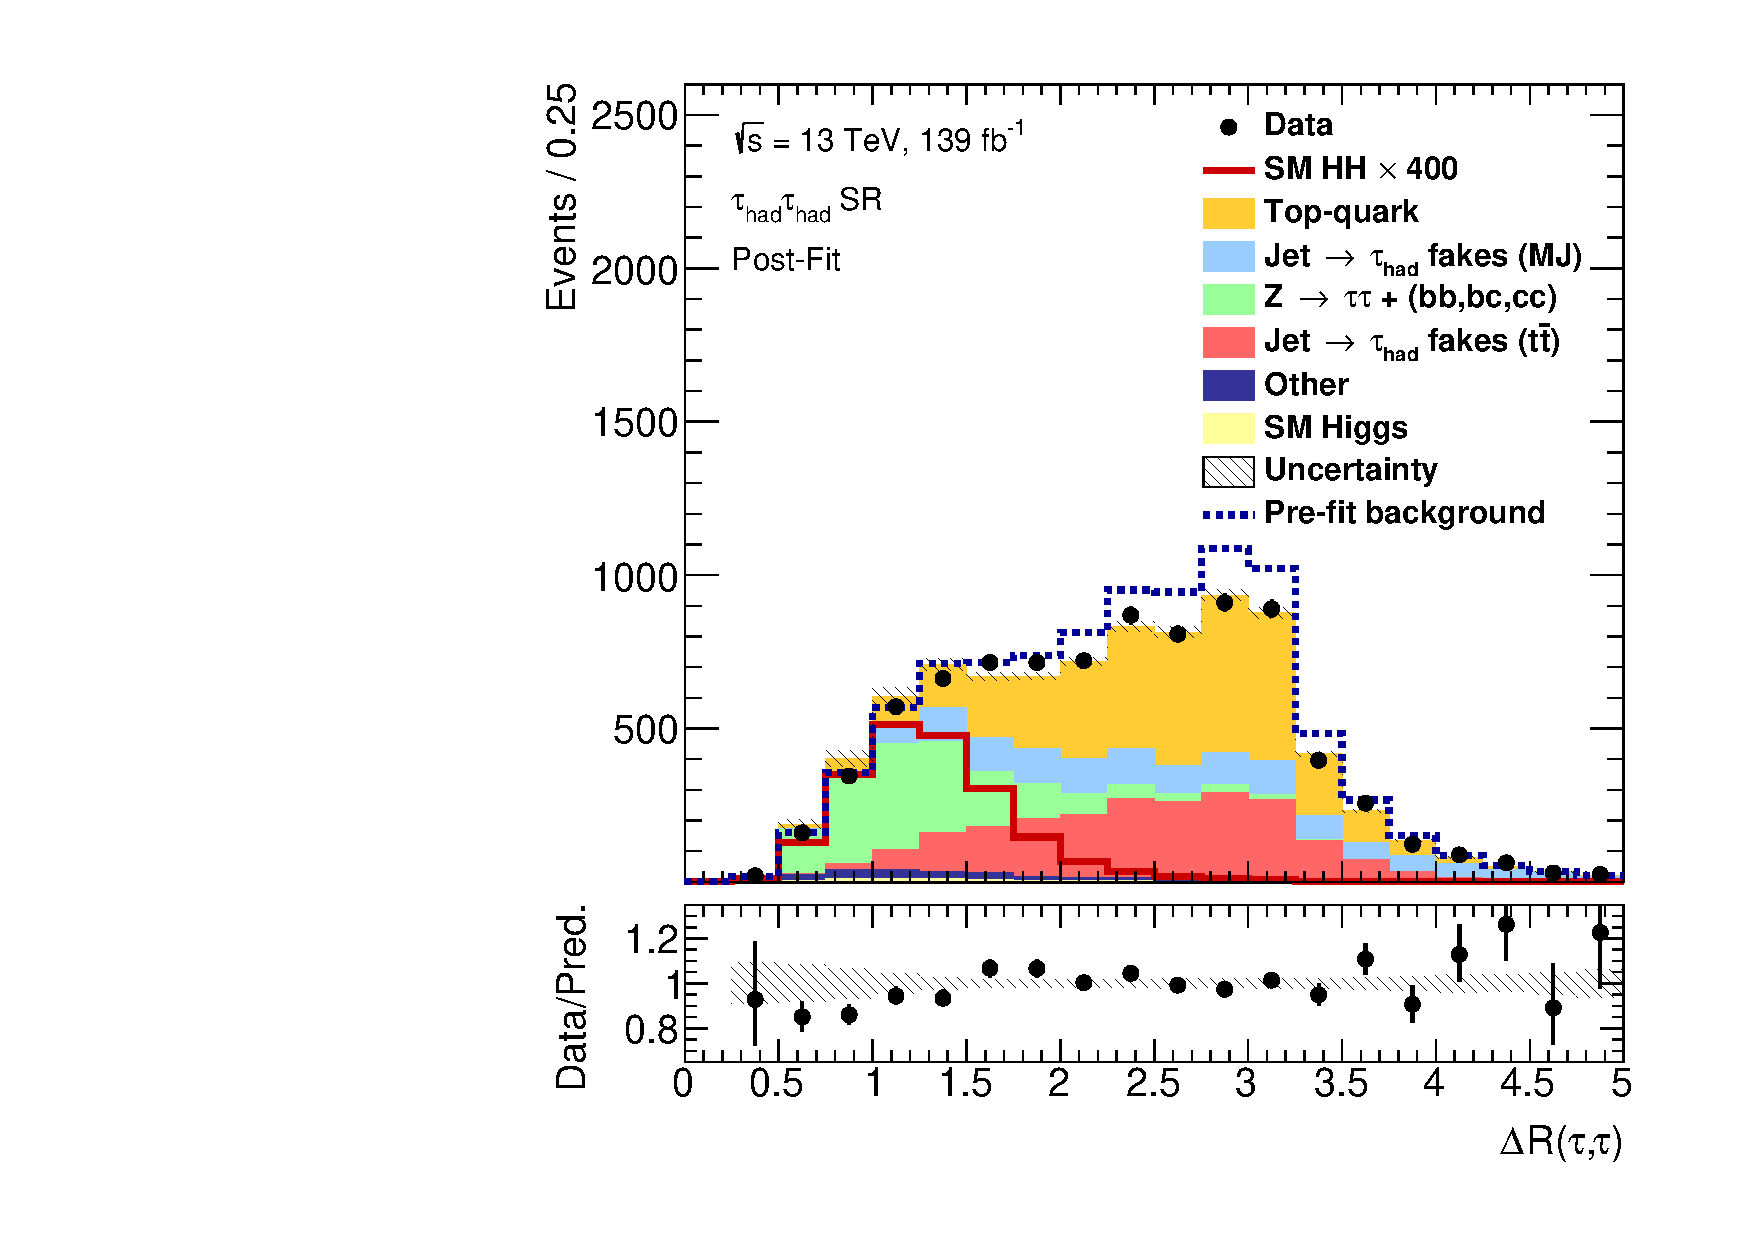
\includegraphics[width=\textwidth]{results_nonres/postfit_mvainputs/Region_BMin0_incJet1_distdRTauTau_J2_Y2015_DLLOS_T2_SpcTauHH_L0_GlobalFit_conditionnal_mu0}
  \end{subfigure}\hfill%
  \begin{subfigure}{0.46\textwidth}
    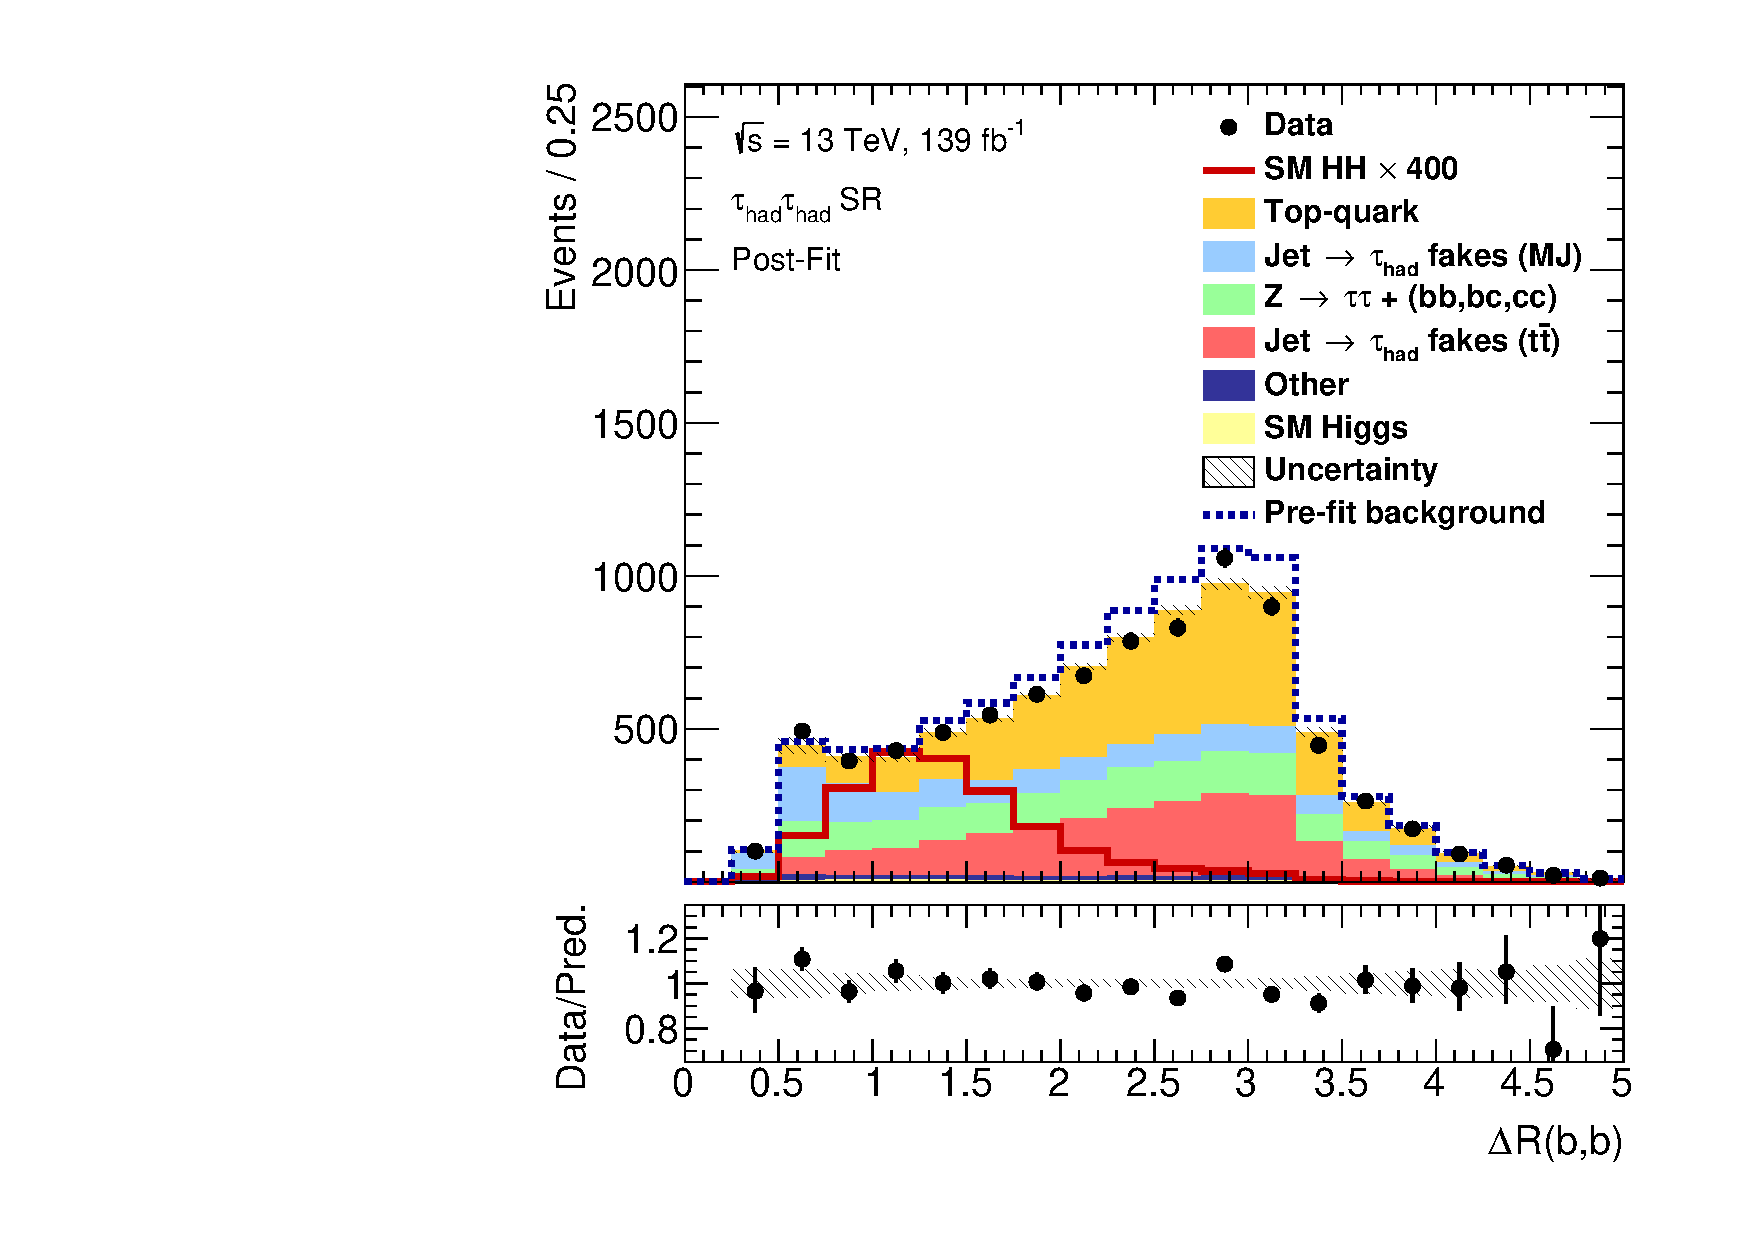
\includegraphics[width=\textwidth]{results_nonres/postfit_mvainputs/Region_BMin0_incJet1_distdRBB_J2_Y2015_DLLOS_T2_SpcTauHH_L0_GlobalFit_conditionnal_mu0}
  \end{subfigure}

  \begin{subfigure}{0.46\textwidth}
    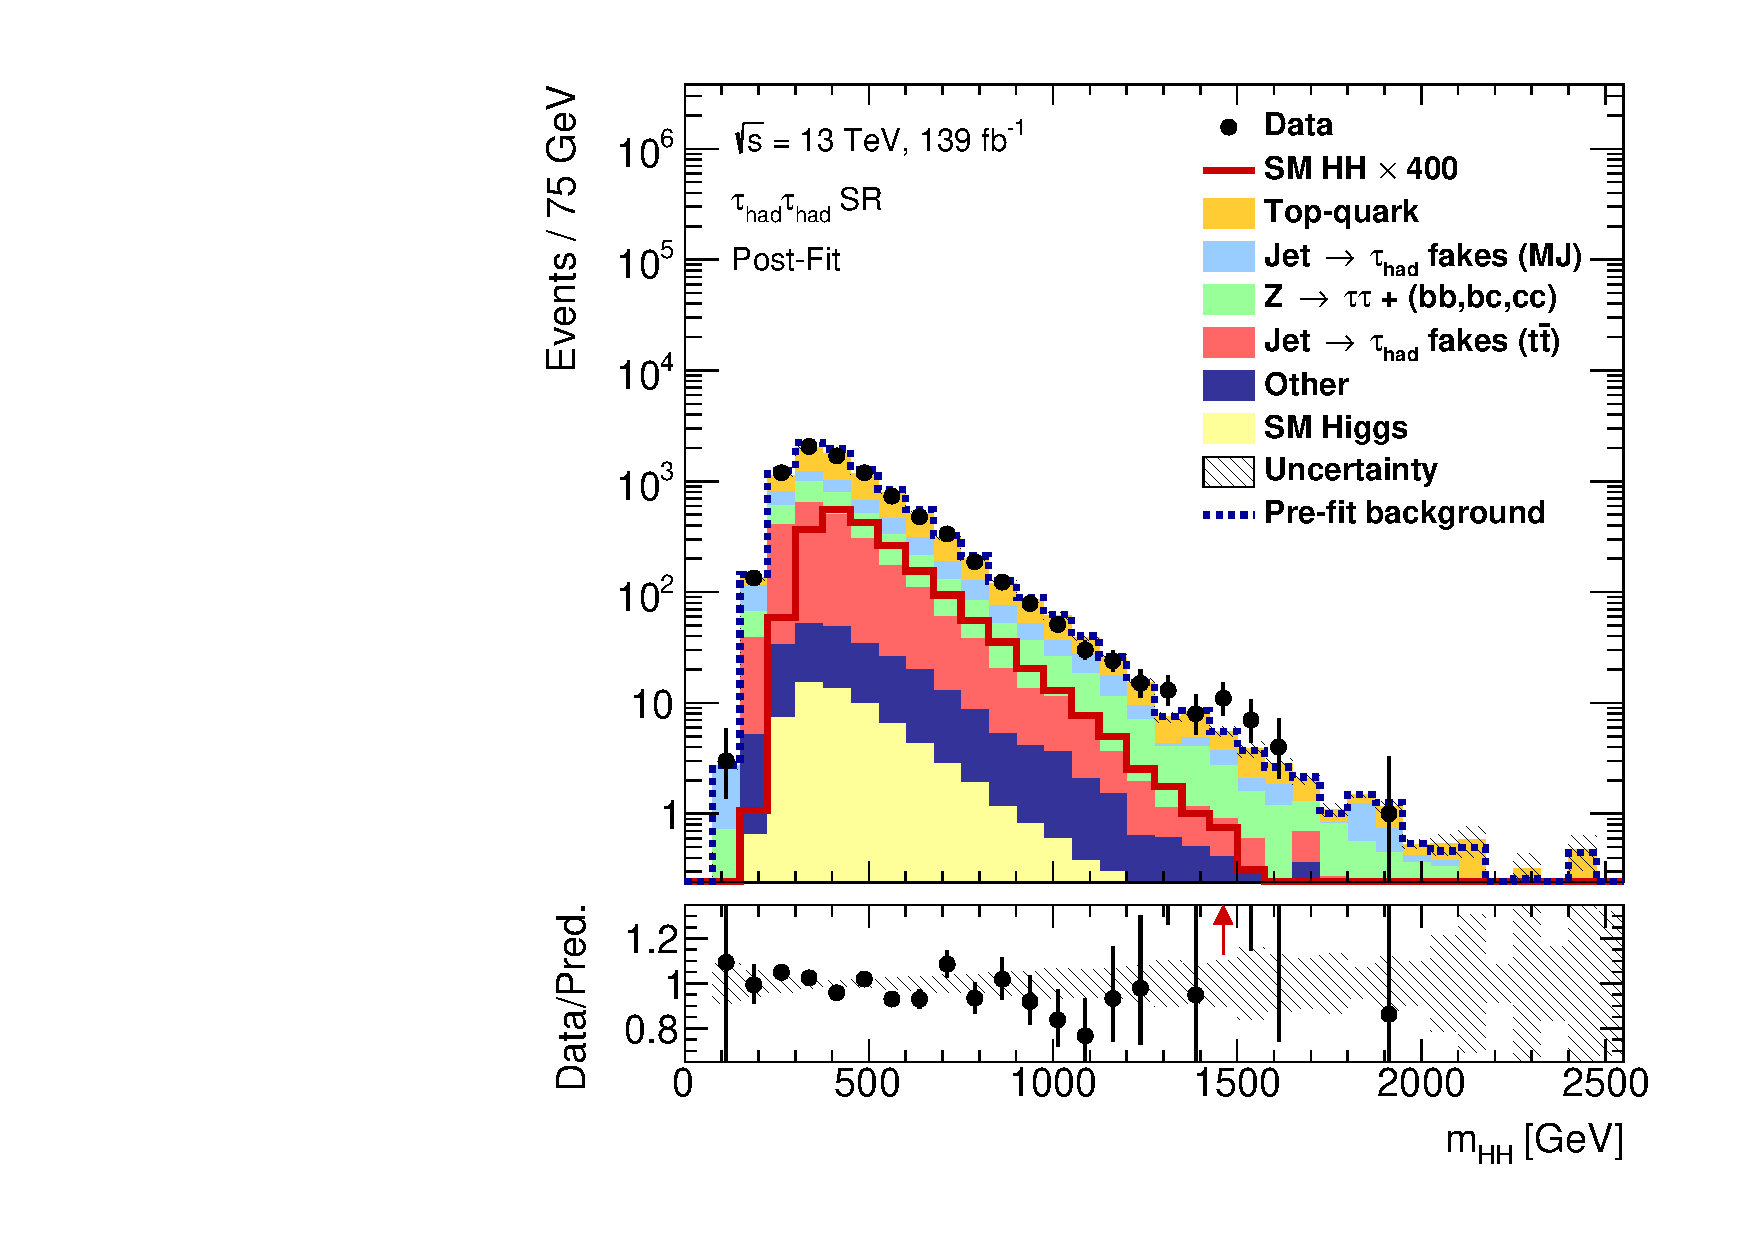
\includegraphics[width=\textwidth]{results_nonres/postfit_mvainputs/Region_BMin0_incJet1_distmHH_J2_Y2015_DLLOS_T2_SpcTauHH_L0_GlobalFit_conditionnal_mu0log}
  \end{subfigure}

  \caption{Distributions of the BDT input variables in the \hadhad
    signal region after the background-only fit of MVA scores and \mll
    in signal and control regions. The expected SM $\HH$ signal is
    overlayed after scaling the normalisation by 400.}
\end{figure}



% q0 (obs): 0.357911
% sig (obs): 0.598257
% pval (obs): 0.274834

% SM (Asimov mu = 1)
% Median significance: 0.667530
% Median pValue: 0.252217

The background-only hypothesis is compared to the alternative of the
background in addition to a positive SM \HH signal with
strength~$\mu$. The likelihood ratio test comparing both hypotheses
yields an observed $p$-value of \SI{27.5}{\percent} (expected
$p$-value of \SI{25.2}{\percent} from the $\mu = 1$ Asimov
dataset). Therefore, the background-only hypothesis cannot be rejected
and thus upper limits on the SM \HH signal strength and cross sections
are placed using the \CLs method.



\todo[inline]{Postfit MVA input plots (hadhad)}
\todo[inline]{Postfit yields: inclusively and in the last (last two) bin(s)?}
\todo[inline]{Postfit norm factors?}

\todo[inline]{Goodness of fit? -> Good fit so set limits.}

\todo[inline]{Postfit ranking: combined, hadhad, lephad}
\todo[inline]{Grouped impact? / Breakdown?}

\begin{table}[htbp]
  \centering

  % Workspaces: comb_2022_01_29
  % ==================
% Channel: combined
% Upper limit on mu:
%         Obs.     -2sigma     -1sigma        Exp.     +1sigma     +2sigma
%     4.700596    2.082483    2.795737    3.879976    5.399804    7.238819

% Upper limit on xsec [fb]:
%         Obs.     -2sigma     -1sigma        Exp.     +1sigma     +2sigma
%     136.6652     61.5679     82.6550    114.7102    159.6434    214.0133

% ==================
% ==================
% Channel: hadhad
% Upper limit on mu:
%         Obs.     -2sigma     -1sigma        Exp.     +1sigma     +2sigma
%     4.951880    2.371052    3.183142    4.417624    6.148054    8.241901

% Upper limit on xsec [fb]:
%         Obs.     -2sigma     -1sigma        Exp.     +1sigma     +2sigma
%     145.1928     70.4159     94.5334    131.1952    182.5858    244.7692

% ==================
% ==================
% Channel: lephad
% Upper limit on mu:
%         Obs.     -2sigma     -1sigma        Exp.     +1sigma     +2sigma
%     9.679448    4.205958    5.646506    7.836325   10.905898   14.620128

% Upper limit on xsec [fb]:
%         Obs.     -2sigma     -1sigma        Exp.     +1sigma     +2sigma
%     281.6663    124.3330    166.9173    231.6509    322.3910    432.1879

% ==================
\begin{tabular}{
  lc
  S[table-format=3.1, round-mode=figures, round-precision=2]
  S[table-format=3.1, round-mode=figures, round-precision=2]
  S[table-format=3.1, round-mode=figures, round-precision=2]
  S[table-format=3.1, round-mode=figures, round-precision=2]
  S[table-format=3.1, round-mode=figures, round-precision=2]
  S[table-format=3.1, round-mode=figures, round-precision=2]
  }
  \toprule
  && {Observed} & {$-2\sigma$} & {$-1\sigma$} & {Expected} & {$+1\sigma$} & {$+2\sigma$} \\
  \midrule
  \multirow{2}{*}{\lephad channel} & {$\xsecggfvbf \, / \, \si{\femto\barn}$} & 281.6663 & 124.3330 & 166.9173 & 231.6509 & 322.3910 & 432.1879 \\
                                   & {$\mu$} & 9.679448 & 4.205958 & 5.646506 & 7.836325 & 10.905898 & 14.620128 \\
  \midrule
  \multirow{2}{*}{\hadhad channel} & {$\xsecggfvbf \, / \, \si{\femto\barn}$} & 145.1928 & 70.4159 & 94.5334 & 131.1952 & 182.5858 & 244.7692 \\
                                   & {$\mu$} & 4.951880 & 2.371052 & 3.183142 & 4.417624 & 6.148054 & 8.241901 \\
  \midrule
  \multirow{2}{*}{Combination}     & {$\xsecggfvbf \, / \, \si{\femto\barn}$} & 136.6652 & 61.5679 & 82.6550 & 114.7102 & 159.6434 & 214.0133 \\
                                   & {$\mu$} & 4.700596 & 2.082483 & 2.795737 & 3.879976 & 5.399804 & 7.238819 \\
  \bottomrule
\end{tabular}

%%% Local Variables:
%%% mode: latex
%%% TeX-master: "../phd_thesis"
%%% End:


  \caption{Upper limits on the total cross section of Higgs pair
    production via ggF and VBF as well as the signal
    strength~$\mu = \sigma_\text{ggF+VBF} /
    \sigma_\text{ggF+VBF}^\text{SM}$ at 95\% $\text{CL}_\text{s}$.}
  \todo[inline]{Make a note somewhere that the cross section upper
    limits are using a different workspace which removes cross section
    uncertainties.}
  \label{tab:limits_non_resonant}
\end{table}


\subsection{Results of the search for resonant production of $HH$}
\label{sec:results_res}

\todo[inline]{Post fit plots of MVAs}
\todo[inline]{Ranking plots: Selected masses combined only}
\todo[inline]{Pull plots? (+Asimov)}



\begin{figure}[htbp]
  \centering

  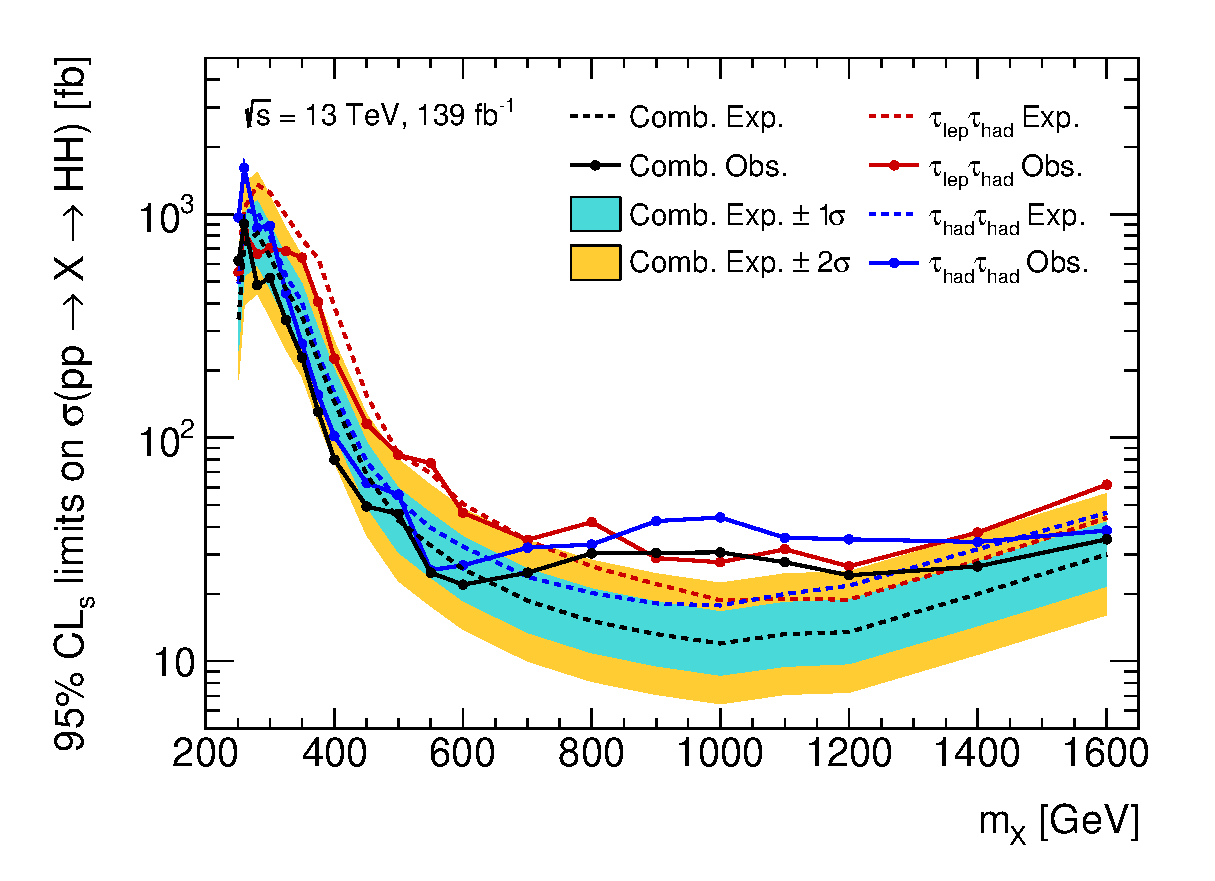
\includegraphics[width=0.65\textwidth]{results/resonant_comb_upper_limits}

  \caption{Upper limits for the resonant search}
  \label{fig:res_upper_limits}
\end{figure}

\begin{figure}[htbp]
  \centering

  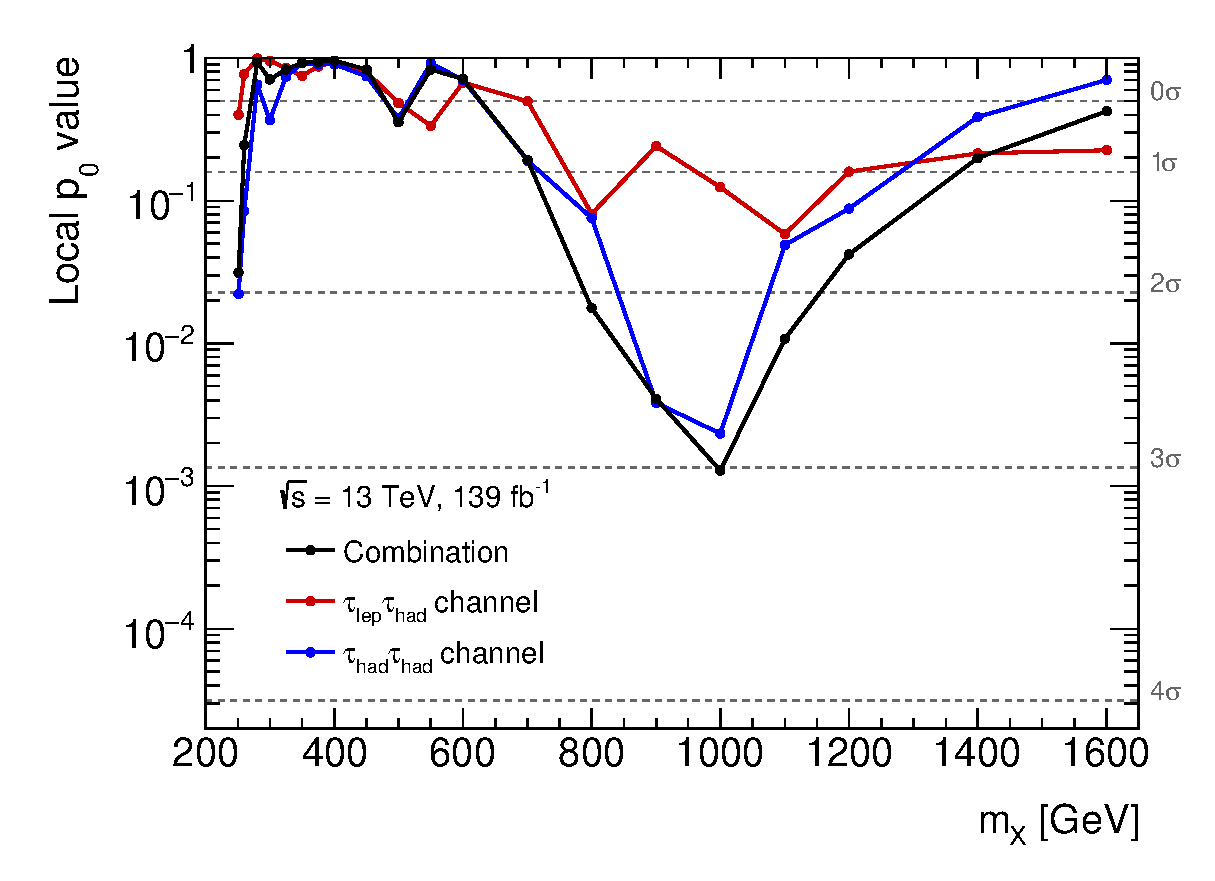
\includegraphics[width=0.65\textwidth]{results/resonant_comb_pvalues}

  \caption{Local pvalue scan}
  \label{fig:local_pvalues}
\end{figure}

\subsection{Global significance estimation of the $\mX = \SI{1000}{\GeV}$ excess}

\subsection{Discussion}

\todo[inline]{What are the limiting factors? Data statistics /
  statistical precision of the bkg estimate (could be improved with a
  better data-driven background estimate).}

\todo[inline]{Systematic uncertainty relatively unimportant at this
  stage.}


\begin{table}[htbp]
  \centering

  \begin{tabular}{lSS}
    \toprule
    & \multicolumn{2}{c}{Expected number of events} \\
    Process & {Last two bins} & {Last bin} \\
    \midrule
    \ZHF & 6.9 & \\
    Single Higgs boson & 6.9 & \\
    \ttbar & 4.6 & \\
    \jettotauhadvis (\ttbar) & 3.4 & \\
    \jettotauhadvis (multi-jet) & 2.2 & \\
    Other & 1.8 & \\
    \midrule
    Total background & & \\
    \midrule
    SM \HH (gluon fusion) & & \\
    SM \HH (VBF) & & \\
    \bottomrule
  \end{tabular}

  \caption{Table of expected yields. The uncertainties are from
    statistical sources only.}
  \todo[inline]{Post-fit yields}
\end{table}


%%% Local Variables:
%%% mode: latex
%%% TeX-master: "../../phd_thesis"
%%% End:
